\documentclass[11pt,a4paper]{article}

% ==================================================================
%  El algoritmo principal del Monoide de Transición
%  Documento académico — Matemática Discreta II
% ==================================================================
\usepackage[utf8]{inputenc}
\usepackage[T1]{fontenc}
\usepackage{babel}
\babelprovide[import,main]{spanish}
\usepackage{mathpazo}
\usepackage[scaled=0.90]{helvet}
\usepackage{microtype}
\usepackage{amsmath,amssymb,amsthm}
\usepackage[a4paper,margin=2.6cm]{geometry}
\usepackage{xcolor}
\usepackage{booktabs}
\usepackage{array}
\usepackage{tikz}
\usetikzlibrary{automata,positioning,arrows.meta,calc}
\usepackage{enumitem}
\usepackage{titlesec}
\usepackage{listings}
\usepackage{pifont}
\usepackage{fancyhdr}
\usepackage[colorlinks=true,linkcolor=accent,urlcolor=accent2,citecolor=accent]{hyperref}

% ---------- Paleta ----------
\definecolor{accent}{HTML}{1F4E79}
\definecolor{accent2}{HTML}{2E7D64}
\definecolor{warn}{HTML}{9A6700}
\definecolor{soft}{HTML}{F4F7FA}
\definecolor{codebg}{HTML}{F7F9FC}
\definecolor{ink}{HTML}{1F2328}
\definecolor{grayrule}{HTML}{C9D3DE}
\color{ink}

% ---------- Títulos ----------
\titleformat{\section}{\sffamily\Large\bfseries\color{accent}}{\thesection.}{0.6em}{}
\titleformat{\subsection}{\sffamily\large\bfseries\color{accent2}}{\thesubsection}{0.6em}{}
\titlespacing*{\section}{0pt}{1.5em}{0.6em}

% ---------- Encabezado / pie ----------
\pagestyle{fancy}\fancyhf{}
\renewcommand{\headrulewidth}{0.4pt}
\renewcommand{\headrule}{\hbox to\headwidth{\color{grayrule}\leaders\hrule height \headrulewidth\hfill}}
\fancyhead[L]{\sffamily\footnotesize\color{accent}Monoide de Transición $\cdot$ El algoritmo principal}
\fancyhead[R]{\sffamily\footnotesize\color{gray}\thepage}
\fancyfoot[C]{\sffamily\footnotesize\color{gray}Proyecto final $\cdot$ Matemática Discreta II}

% ---------- Teoremas ----------
\newtheoremstyle{acc}{}{}{\itshape}{}{\sffamily\bfseries\color{accent}}{.}{.5em}{}
\theoremstyle{acc}
\newtheorem{teorema}{Teorema}
\newtheorem{definicion}{Definición}

% ---------- Cajas de realce ----------
\newsavebox{\cboxbuf}
\newenvironment{callout}[2]{%
  \def\cc{#1}%
  \begin{lrbox}{\cboxbuf}%
  \begin{minipage}{\dimexpr\linewidth-2.8em\relax}%
  \smallskip{\sffamily\bfseries\color{#1}#2}\par\smallskip
}{%
  \par\smallskip\end{minipage}\end{lrbox}%
  \par\medskip\noindent
  \begin{tikzpicture}
    \node[draw=\cc!75,line width=0.8pt,rounded corners=5pt,
          fill=\cc!7,inner sep=11pt]{\usebox{\cboxbuf}};
  \end{tikzpicture}\par\medskip
}

% ---------- Estilo de pseudocódigo ----------
\lstdefinestyle{algo}{
  basicstyle=\small\ttfamily,
  keywordstyle=\bfseries\color{accent},
  commentstyle=\itshape\color{accent2},
  mathescape=true,
  escapeinside={(@}{@)},
  numbers=left, numberstyle=\scriptsize\color{gray}, numbersep=10pt,
  frame=leftline, framerule=1.4pt, rulecolor=\color{accent!55},
  backgroundcolor=\color{codebg},
  xleftmargin=20pt, framexleftmargin=16pt,
  aboveskip=1em, belowskip=1em,
  morekeywords={Entrada,Salida,para,cada,en,mientras,si,entonces,sino,
    devolver,agregar,nuevo,vacío,vacia,funcion,fin,hacer,no,y,o,con},
}

\newcommand{\code}[1]{{\ttfamily #1}}
\newcommand{\cmark}{{\color{accent2}\ding{51}}}
\newcommand{\xmark}{{\color{warn}\ding{55}}}
\setlist[itemize]{leftmargin=1.4em,itemsep=2pt,topsep=3pt}
\setlist[enumerate]{leftmargin=1.7em,itemsep=2pt,topsep=3pt}

% ==================================================================
\begin{document}

% ---------- Portada ----------
\begin{titlepage}
\centering
\vspace*{1.6cm}
{\color{accent}\rule{\linewidth}{1.4pt}}\\[1.1cm]
{\sffamily\bfseries\color{accent}\Huge El algoritmo principal\\[0.35cm]
 del Monoide de Transición}\\[0.7cm]
{\Large\itshape De un lenguaje a su estructura de álgebra abstracta}\\[0.5cm]
{\large Autómatas, expresiones regulares y el monoide de transición $M(A)$}\\[1.0cm]
{\color{accent}\rule{\linewidth}{1.4pt}}\\[1.4cm]

\begin{minipage}{0.85\linewidth}\centering\itshape\color{ink}
Documento explicativo del proyecto final. Describe, paso a paso y de forma
autocontenida, cómo el programa transforma una regla que acepta o rechaza
palabras en un objeto algebraico finito, y cómo lee en él la estructura de grupo
o de monoide del lenguaje. Pensado para leerse sin conocimientos previos de
teoría de autómatas.
\end{minipage}\\[1.6cm]

{\large\sffamily Proyecto integrador}\\[0.2cm]
{\sffamily\color{accent2}Matemática Discreta II \; \& \; Teoría de la Computación}\\[0.8cm]
{\small Marco teórico basado únicamente en dos fuentes:\\
D.~Saracino, \textit{Abstract Algebra: A First Course}\; (álgebra) \; y\\
R.~De Castro Korgi, \textit{Introducción a la Teoría de la Computación}\; (2024).}
\vfill
\end{titlepage}

\tableofcontents
\thispagestyle{fancy}
\vspace{1em}

% ==================================================================
\section{¿Qué problema resuelve el algoritmo?}

Un \textbf{lenguaje} es, simplemente, una regla que separa las palabras en dos
grupos: las que \emph{acepta} y las que \emph{rechaza}. Por ejemplo, «las cadenas
binarias con un número par de unos» o «las que terminan en \code{01}».

La teoría clásica de autómatas responde a la pregunta \emph{«¿cómo reconozco este
lenguaje con una máquina?»}. Este proyecto añade una segunda pregunta, más
profunda y de naturaleza \textbf{algebraica}:

\begin{callout}{accent}{La pregunta central del proyecto}
Dado un lenguaje, ¿cuál es su \textbf{estructura de álgebra abstracta}? ¿Es un
grupo? Si lo es, ¿cuál ($\mathbb{Z}/n\mathbb{Z}$, el grupo de Klein $V_4$, el
simétrico $S_3$\ldots)? ¿Es abeliano, cíclico? ¿O es un monoide aperiódico?
\end{callout}

El puente entre ambos mundos es un objeto llamado el \textbf{monoide de
transición} $M(A)$, y \emph{construirlo y analizarlo} es el algoritmo principal
que describe este documento. Todo lo demás (leer una expresión regular,
construir el autómata, minimizarlo) es la maquinaria necesaria para llegar hasta
él.

% ==================================================================
\section{Panorama: el flujo completo}

El programa encadena cinco etapas. Las tres primeras producen un autómata; las
dos últimas son el corazón algebraico.

\begin{center}
\footnotesize\sffamily
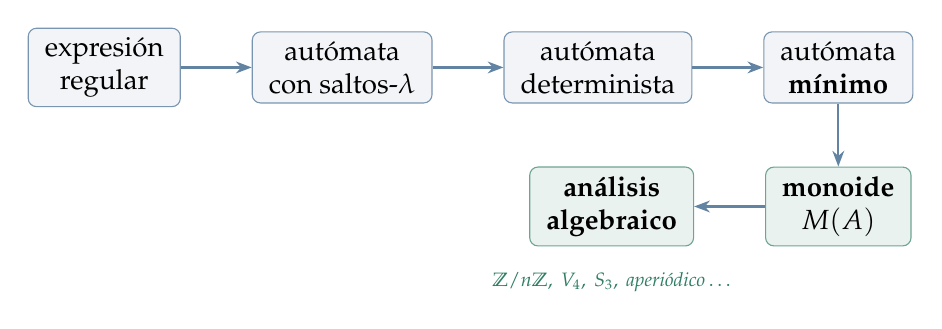
\begin{tikzpicture}[
  node distance=6mm and 9mm,
  box/.style={draw=accent!60,fill=accent!6,rounded corners=3pt,
              minimum height=8mm,inner xsep=6pt,align=center},
  core/.style={draw=accent2!70,fill=accent2!10,rounded corners=3pt,
              minimum height=8mm,inner xsep=6pt,align=center,font=\bfseries},
  fl/.style={-{Stealth[length=2mm]},accent!70,thick}]
\node[box] (rx) {expresión\\regular};
\node[box,right=of rx] (nfa) {autómata\\con saltos-$\lambda$};
\node[box,right=of nfa] (dfa) {autómata\\determinista};
\node[box,right=of dfa] (min) {autómata\\\textbf{mínimo}};
\node[core,below=8mm of min] (mon) {monoide\\$M(A)$};
\node[core,left=of mon] (an) {análisis\\algebraico};
\draw[fl] (rx)--(nfa); \draw[fl] (nfa)--(dfa); \draw[fl] (dfa)--(min);
\draw[fl] (min)--(mon); \draw[fl] (mon)--(an);
\node[below=2mm of an,font=\itshape\scriptsize,accent2] {$\mathbb{Z}/n\mathbb{Z},\ V_4,\ S_3,\ \text{aperiódico}\ldots$};
\end{tikzpicture}
\end{center}

\begin{enumerate}
  \item \textbf{Parseo.} Leer la expresión regular y entenderla como una
        estructura jerárquica (un árbol).
  \item \textbf{Construcción del AFN-$\lambda$} (Teorema de Kleene, §2.12).
        Convertir ese árbol en un autómata con transiciones vacías
        ($\lambda$): fácil de armar, imposible de usar directamente.
  \item \textbf{Determinización y minimización.} Eliminar la ambigüedad y luego
        fusionar estados indistinguibles hasta obtener el autómata
        \textbf{mínimo}.
  \item \textbf{Construcción del monoide $M(A)$.} \emph{(algoritmo principal)}
  \item \textbf{Análisis algebraico.} \emph{(algoritmo principal)}
\end{enumerate}

Este documento resume las etapas 1--3 (Sección~\ref{sec:auto}) y desarrolla en
detalle las etapas 4--5 (Secciones~\ref{sec:mon} y~\ref{sec:an}), que son la
contribución del proyecto.

% ==================================================================
\section{Preliminares accesibles}\label{sec:auto}

\subsection{Autómata finito determinista (AFD)}
Un AFD es la máquina reconocedora más simple. Formalmente es una quíntupla
$A=(Q,\Sigma,\delta,q_0,F)$, pero conviene leerla en palabras llanas:

\begin{itemize}
  \item $Q$: un conjunto finito de \textbf{estados} (los «focos»; en cada
        instante hay exactamente uno activo).
  \item $\Sigma$: el \textbf{alfabeto}, las letras admitidas.
  \item $\delta:Q\times\Sigma\to Q$: la \textbf{función de transición}, que dado
        «estado actual» y «letra leída» dice el «estado siguiente». Es total y
        \emph{determinista}: para cada par hay \emph{una} respuesta.
  \item $q_0\in Q$: el estado \textbf{inicial}.
  \item $F\subseteq Q$: los estados \textbf{de aceptación} (los «buenos»).
\end{itemize}

La máquina lee la palabra de izquierda a derecha, aplicando $\delta$ letra a
letra. Extendemos $\delta$ a palabras completas con $\hat\delta(q,w)$ = «estado
donde termino si arranco en $q$ y leo toda la palabra $w$». La palabra $w$ se
\textbf{acepta} si $\hat\delta(q_0,w)\in F$.

\subsection{De la regex al autómata mínimo (en breve)}
\begin{itemize}
  \item La \textbf{construcción del AFN-$\lambda$} (Teorema de Kleene, §2.12)
        traduce cada operación de la regex (unión, concatenación, estrella de
        Kleene) en un pequeño autómata con transiciones $\lambda$ (saltos que
        no consumen letra), y los pega entre sí.
  \item La \textbf{construcción de subconjuntos} elimina la no-determinación:
        un \emph{conjunto} de estados del autómata ambiguo se comporta como un
        \emph{único} estado determinista.
  \item La \textbf{minimización} (refinamiento de particiones) fusiona los
        estados que son indistinguibles: aquellos desde los cuales
        \emph{exactamente las mismas palabras futuras} llevan a la aceptación.
\end{itemize}

Retendremos una sola cosa de esta etapa, pero es crucial:

\begin{callout}{warn}{Por qué el autómata debe ser mínimo}
Solo cuando el AFD es \textbf{mínimo}, su monoide de transición $M(A)$ es un
\textbf{invariante del lenguaje} $L(A)$ —depende de $L$, no de cómo dibujemos la
máquina—. Esto lo garantiza el Teorema de Myhill--Nerode de De Castro
(Sección~\ref{sec:teoria}).
\end{callout}

% ==================================================================
\section{Algoritmo principal, parte 1: construir \texorpdfstring{$M(A)$}{M(A)}}\label{sec:mon}

\subsection{La idea: cada palabra es una transformación}
Fijemos el AFD mínimo. La observación de partida es sencilla pero poderosa:
\emph{cada palabra reordena los estados}. Con precisión, la palabra $w$ induce
una función del conjunto de estados en sí mismo,
\[
  f_w : Q \longrightarrow Q, \qquad f_w(q) = \hat\delta(q,w),
\]
que dice: «si empiezo en el estado $q$ y leo $w$, termino en $f_w(q)$». A una
función de $Q$ en $Q$ la llamamos una \textbf{transformación} de estados.

\begin{callout}{accent2}{Ejemplos de transformación}
$f_\lambda$ (palabra vacía) es la \textbf{identidad}: no mueve nada.
$f_a$ para una sola letra $a$ es «seguir la flecha $a$» desde cada estado.
Encadenar palabras corresponde a \emph{componer} funciones:
$f_{uv} = f_u$ seguida de $f_v$.
\end{callout}

\subsection{El objeto: el monoide de transición}
\begin{definicion}[Monoide de transición]
El \textbf{monoide de transición} de $A$ es el conjunto de \emph{todas} las
transformaciones inducidas por palabras,
\[
  M(A) = \{\, f_w : w\in\Sigma^* \,\},
\]
con la operación de \textbf{composición} de funciones y elemento neutro
$f_\lambda$.
\end{definicion}

Es un \emph{monoide} porque la composición es asociativa y tiene neutro. Y es
\textbf{finito}: hay a lo sumo $|Q|^{|Q|}$ funciones de $Q$ en $Q$, de modo que
por más palabras que existan (infinitas), las transformaciones distintas son un
número finito. Ese es el milagro que hace posible el análisis:

\begin{callout}{accent}{Compresión de lo infinito}
El homomorfismo $\varphi:\Sigma^*\to M(A)$, $w\mapsto f_w$, colapsa las
\textbf{infinitas} palabras sobre un conjunto \textbf{finito} de
transformaciones. Dos palabras caen en el mismo elemento exactamente cuando
«hacen lo mismo» a todos los estados. Ese conjunto finito es una huella digital
completa del lenguaje.
\end{callout}

\subsection{Un detalle de convención (composición izquierda-a-derecha)}
El programa compone en el orden en que se leen las palabras:
\[
  (f\cdot g)(q) = g\big(f(q)\big).
\]
Con esta convención, leer $u$ y luego $v$ es $f_u\cdot f_v$, y por tanto
$\varphi(uv)=\varphi(u)\cdot\varphi(v)$: $\varphi$ es un \textbf{homomorfismo}
(y no un anti-homomorfismo). Esto es lo que permitirá, más adelante, aplicar
limpiamente el teorema de isomorfismo de Saracino (§12).

\subsection{La construcción por cierre (BFS)}
No se enumeran las $|Q|^{|Q|}$ funciones posibles: se \textbf{generan} a partir
de las transformaciones de una sola letra, $\{f_a : a\in\Sigma\}$, cerrando bajo
composición mediante un recorrido en anchura (BFS).

\begin{lstlisting}[style=algo,caption={},captionpos=b]
Entrada: AFD minimo $A=(Q,\Sigma,\delta,q_0,F)$
Salida:  el conjunto $M(A)$ de transformaciones distintas
         (con la palabra mas corta que produce cada una)

$f_\lambda \leftarrow$ identidad sobre $Q$
$M \leftarrow \{\, f_\lambda \,\}$              // elementos ya descubiertos
$cola \leftarrow [\, f_\lambda \,]$             // pendientes por expandir
para cada $a\in\Sigma$: precomputar $f_a$        // "seguir la flecha $a$"

mientras la $cola$ no este vacia hacer
   $f \leftarrow$ sacar frente de la $cola$
   para cada letra $a\in\Sigma$ hacer
       $g \leftarrow f \cdot f_a$               // componer: leer $a$ despues de $f$
       si $g \notin M$ entonces                 // transformacion nueva?
           agregar $g$ a $M$
           agregar $g$ a la $cola$
       fin si
   fin para
fin mientras
devolver $M$
\end{lstlisting}

\noindent\textbf{Por qué funciona y por qué termina.}
Cada elemento nuevo se descubre componiendo uno ya conocido con un generador
$f_a$; como los generadores producen todo el monoide, el BFS encuentra
\emph{todos} los elementos. Y como $|M(A)|\le |Q|^{|Q|}$ es finito, no pueden
aparecer elementos nuevos para siempre: la cola se vacía. Comparar «$g\notin M$»
se hace con una \textbf{clave canónica} de cada transformación (la lista
ordenada de sus pares $q\mapsto f(q)$), de modo que dos funciones iguales
reciben la misma clave. El registro de la «palabra más corta» que genera cada
elemento es lo que permite luego decir, por ejemplo, que un grupo cíclico
\emph{está generado por la palabra} \code{1}.

% ==================================================================
\section{Algoritmo principal, parte 2: leer la estructura}\label{sec:an}

\subsection{La tabla de Cayley}
Con los $n=|M(A)|$ elementos ya en mano, se construye su \textbf{tabla de
composición} (o tabla de Cayley): una matriz $n\times n$ donde la casilla
$(i,j)$ guarda el índice de $f_i\cdot f_j$. Es, literalmente, la «tabla de
multiplicar» del monoide. A partir de ella, \emph{todas} las propiedades
algebraicas son lecturas baratas de la tabla:

\begin{center}
\renewcommand{\arraystretch}{1.35}
\begin{tabular}{@{}>{\bfseries}p{3.5cm} p{10.5cm}@{}}
\toprule
\normalfont\textbf{Propiedad} & \textbf{Cómo se decide sobre la tabla} \\
\midrule
Idempotentes & elementos con $f\cdot f = f$ (la diagonal apunta a sí misma). \\
Unidades $U(M)$ & elementos \emph{invertibles}: existe $g$ con
   $f\cdot g = g\cdot f = f_\lambda$. \\
¿Es grupo? & \emph{todo} elemento es una unidad ($|U(M)|=n$). \\
¿Abeliano? & la tabla es simétrica: $f_i\cdot f_j = f_j\cdot f_i$ para todo par. \\
Centro $Z(M)$ & elementos que conmutan con todos. \\
¿Cíclico? (grupo) & existe un elemento cuyas potencias sucesivas recorren los
   $n$ elementos: un \emph{generador}. \\
¿Aperiódico? & para todo $x$, alguna potencia se estabiliza:
   $x^{k}=x^{k+1}$ (no hay ciclos no triviales). \\
\bottomrule
\end{tabular}
\end{center}

\subsection{Qué significan estas propiedades}
Aquí es donde Matemática Discreta II y Teoría de la Computación se encuentran:

\begin{itemize}
  \item Si $M(A)$ es un \textbf{grupo}, el programa lo \textbf{clasifica}: trivial,
        $\mathbb{Z}/n\mathbb{Z}$ (cíclico), $V_4=\mathbb{Z}/2\mathbb{Z}\times
        \mathbb{Z}/2\mathbb{Z}$ (Klein), $S_3$, etc. El grupo abstracto
        \emph{es} la estructura de conteo del lenguaje.
  \item Si \textbf{no} es grupo pero es \textbf{aperiódico}, significa que al
        iterar cualquier palabra su transformación se estabiliza
        ($x^{k}=x^{k+1}$, Saracino §3): $M(A)$ no contiene ningún subgrupo no
        trivial. El lenguaje solo «detecta patrones», sin contar en ciclos.
\end{itemize}

% ==================================================================
\section{Un ejemplo completo, de principio a fin}

Tomemos el lenguaje $L=\{$cadenas binarias con un número \emph{par} de unos$\}$.
Su AFD mínimo tiene dos estados:

\begin{center}
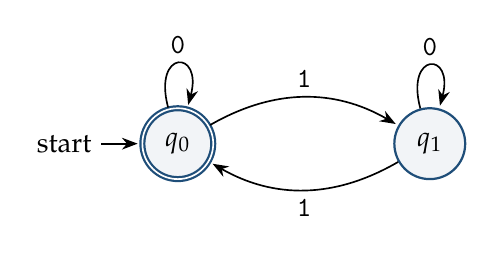
\begin{tikzpicture}[->,>=Stealth,shorten >=1pt,node distance=3.2cm,semithick,
   every state/.style={draw=accent,fill=accent!6,thick,minimum size=9mm}]
  \node[state,initial,accepting] (q0) {$q_0$};
  \node[state] (q1) [right of=q0] {$q_1$};
  \path (q0) edge[bend left]  node[above]{\code{1}} (q1)
        (q1) edge[bend left]  node[below]{\code{1}} (q0)
        (q0) edge[loop above] node{\code{0}} (q0)
        (q1) edge[loop above] node{\code{0}} (q1);
\end{tikzpicture}
\end{center}

\noindent con $q_0$ = «\#unos par» (inicial y de aceptación) y $q_1$ = «\#unos
impar». La función de transición es $\delta(q_0,0)=q_0$, $\delta(q_0,1)=q_1$,
$\delta(q_1,0)=q_1$, $\delta(q_1,1)=q_0$.

\paragraph{Paso 1: las transformaciones.} Calculamos qué hace cada letra.
\[
  f_\lambda=\begin{pmatrix}q_0\mapsto q_0\\ q_1\mapsto q_1\end{pmatrix}\!,\quad
  f_0=\begin{pmatrix}q_0\mapsto q_0\\ q_1\mapsto q_1\end{pmatrix}\!,\quad
  f_1=\begin{pmatrix}q_0\mapsto q_1\\ q_1\mapsto q_0\end{pmatrix}\!.
\]
Observamos que $f_0$ es la \textbf{identidad} (leer un cero no mueve nada), luego
$f_0=f_\lambda$. Y $f_1$ es el \textbf{intercambio} de los dos estados.
Componiendo, $f_{11}=f_1\cdot f_1=f_\lambda$ (intercambiar dos veces vuelve al
inicio). El BFS no encuentra nada más:
\[
  \boxed{\,M(A)=\{\, e,\ s \,\}\,}\qquad
  e=f_\lambda\ (\text{identidad}),\quad s=f_1\ (\text{intercambio}).
\]

\paragraph{Paso 2: la tabla de Cayley.}
\begin{center}
\renewcommand{\arraystretch}{1.3}
\begin{tabular}{c|cc}
$\cdot$ & $e$ & $s$ \\ \hline
$e$ & $e$ & $s$ \\
$s$ & $s$ & $e$ \\
\end{tabular}
\end{center}

\paragraph{Paso 3: lectura de la estructura.}
\begin{itemize}
  \item \textbf{Idempotentes:} solo $e$ (pues $s\cdot s=e\neq s$).
  \item \textbf{Unidades:} ambas ($e^{-1}=e$, $s^{-1}=s$). Como $|U(M)|=2=n$,
        \textbf{es un grupo}. \cmark
  \item \textbf{Abeliano:} sí (la tabla es simétrica). \textbf{Cíclico:} sí,
        generado por $s$, es decir, por la palabra \code{1}. \cmark
  \item \textbf{Aperiódico:} no, porque $s^1=s,\ s^2=e,\ s^3=s,\dots$ nunca se
        estabiliza. \xmark
\end{itemize}

\begin{callout}{accent}{Conclusión del ejemplo}
$M(A)$ es el grupo cíclico de dos elementos, $M(A)\cong\mathbb{Z}/2\mathbb{Z}$,
generado por la palabra \code{1}. Es el mismo objeto matemático que un
interruptor de luz o que la suma de paridades ($\text{par}+\text{impar}$). La
estructura algebraica \emph{es} la esencia de «contar unos módulo 2».
\end{callout}

% ==================================================================
\section{Fundamento teórico}\label{sec:teoria}

Dos resultados sostienen la corrección y el significado del algoritmo, uno de
cada libro del curso. Los enunciamos de forma accesible.

\begin{teorema}[Myhill--Nerode; De Castro §2.15]
Un lenguaje $L$ es regular si y solo si la relación «tener el mismo futuro»
sobre las palabras tiene un número \emph{finito} de clases. Esas clases son
exactamente los estados del \textbf{AFD mínimo}, que por tanto es único.
\end{teorema}
\noindent Consecuencia para el algoritmo: al minimizar antes de construir
$M(A)$, garantizamos que $M(A)$ es un \textbf{invariante del lenguaje} $L$, y no
un artefacto que dependa del dibujo particular de la máquina.

\begin{teorema}[Teorema de isomorfismo; Saracino §12]
Para un homomorfismo $\varphi$ con dominio adecuado,
\[
  \Sigma^*\big/\ker(\varphi)\ \cong\ M(A).
\]
\end{teorema}
\noindent Es decir: agrupar todas las palabras por «hacen lo mismo» (el núcleo
$\ker\varphi$) y quedarse con las clases produce, salvo isomorfismo, el propio
$M(A)$. Saracino enuncia este teorema para \emph{grupos} (§12); aquí lo
aplicamos, en el mismo espíritu, al homomorfismo de monoides
$\varphi:\Sigma^*\to M(A)$ —esa adaptación es parte del aporte del proyecto—.

\begin{definicion}[Aperiodicidad; a partir de Saracino §3]
$M(A)$ es \textbf{aperiódico} si para todo elemento $x$ alguna potencia se
estabiliza: existe $k$ con $x^{k}=x^{k+1}$. Equivale a que $M(A)$ no contenga
ningún subgrupo no trivial.
\end{definicion}
\noindent La etiqueta «aperiódico» de la página se calcula exactamente con esta
definición, usando las potencias de un elemento (Saracino §3); no requiere
ninguna fuente fuera de los dos textos del curso.

% ==================================================================
\section{La segunda vía: Máquinas de Turing y la frontera de lo regular}

La página ofrece un segundo generador: describes un lenguaje (por ejemplo
$a^nb^nc^n$) y se construye una \textbf{Máquina de Turing} que lo decide,
animando su cinta paso a paso. El vínculo con el álgebra es honesto sobre sus
límites:

\begin{itemize}
  \item Si el lenguaje resulta \textbf{regular} (se describe con \code{regex}\ldots),
        se construye su AFD mínimo y se aplica \emph{el mismo} análisis de las
        Secciones~\ref{sec:mon} y~\ref{sec:an} (Teorema~6.1.1 del libro: todo
        lenguaje regular es Turing-decidible).
  \item Si el lenguaje \textbf{no es regular} (como $a^nb^n$, los palíndromos o
        $ww$), no hay AFD finito y su monoide de transición sería
        \textbf{infinito}; el programa lo indica
        explícitamente y explica por qué la construcción finita no aplica. Muestra,
        así, la frontera precisa que la teoría predice.
\end{itemize}

% ==================================================================
\section{Complejidad y garantías}

Sea $n=|M(A)|$ el tamaño del monoide y $|Q|$ el número de estados del AFD mínimo.

\begin{itemize}
  \item \textbf{Construcción (BFS):} se generan $n$ elementos; cada composición
        cuesta $O(|Q|)$ y cada elemento se prueba contra los ya vistos vía su
        clave canónica. En conjunto, del orden de $O\big(n\,|\Sigma|\,|Q|\big)$
        más el coste de las búsquedas.
  \item \textbf{Análisis (tabla de Cayley):} construirla es $O(n^2\,|Q|)$; sobre
        ella, cada propiedad (grupo, abeliano, centro, idempotentes,
        aperiodicidad) es un recorrido de $O(n^2)$.
  \item \textbf{Cota y salvaguarda:} $n\le |Q|^{|Q|}$. Como esta cota crece muy
        rápido, el programa impone un tope defensivo y, si se supera, informa que
        el monoide es demasiado grande para construirse en el navegador, en lugar
        de bloquearse.
\end{itemize}

\begin{callout}{accent2}{El algoritmo en una frase}
Cada palabra induce una transformación de los estados; el conjunto finito de
transformaciones distintas, cerrado por composición, es el monoide $M(A)$; su
tabla de Cayley revela si el lenguaje es, en el fondo, un grupo (y cuál) o un
monoide aperiódico. Myhill--Nerode garantiza que ese objeto es \emph{el}
invariante canónico del lenguaje.
\end{callout}

% ==================================================================
\section*{\sffamily\color{accent}Referencias}
\addcontentsline{toc}{section}{Referencias}
El marco teórico se apoya \textbf{únicamente} en estos dos textos:

\begin{itemize}[leftmargin=1.4em]
  \item \textbf{D.~Saracino}, \textit{Abstract Algebra: A First Course},
        2.ª ed., Waveland Press, 2008. \emph{Álgebra:} operación binaria y
        monoide (§1), grupos (§2), potencias / cíclicos / $\mathbb{Z}/n\mathbb{Z}$
        y aperiodicidad (§3), productos directos y $V_4$ (§5, §13), funciones y
        composición (§6), grupos simétricos $S_3$ (§7), relaciones de
        equivalencia (§8), homomorfismos (§11) y teorema de isomorfismo (§12).
  \item \textbf{R.~De Castro Korgi}, \textit{Introducción a la Teoría de la
        Computación}, Universidad Nacional de Colombia, 2024. \emph{Computación:}
        expresiones regulares (§2.2), AFD/AFN/AFN-$\lambda$ y Kleene
        (§2.6--2.13), Myhill--Nerode (§2.15), minimización (§2.16), no
        regularidad (§3.1) y Máquinas de Turing (§6.1--6.2, Teorema~6.1.1).
\end{itemize}

\noindent El \textbf{monoide de transición} $M(A)$ es una construcción propia
del proyecto que combina ambas fuentes; no aparece con ese nombre en ninguno de
los dos libros.

\end{document}
